\begin{frame}
    \begin{centering}
        \vskip5ex plus 1filll
        {\usebeamerfont{title page title}\usebeamercolor[fg]{title page} Hysteresis\\[1.5ex]}
        \vskip0pt plus 1filll
    \end{centering}
\end{frame}

\begin{frame}{Hysteresis}
    \begin{columns}
        \begin{column}{0.5\linewidth}
            \begin{itemize}
                \item Stateful nonlinearity that describes magnetisation
                (magnetic tape, transformers, \dots)
                \item Also models processes in civil engineering,
                economics, and more
            \end{itemize}
        \end{column}
        \begin{column}{0.5\linewidth}
            \begin{figure}
                \centering
                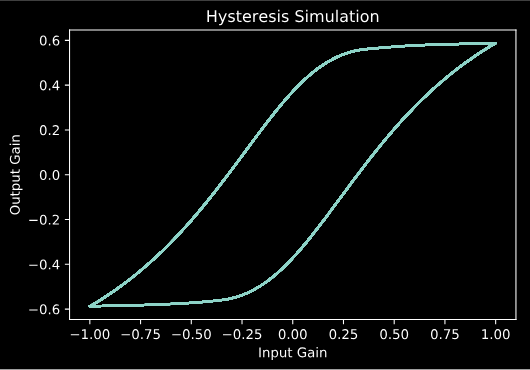
\includegraphics[width=2.5in]{../Hysteresis/Pics/First_Sim}
            \end{figure}
        \end{column}
    \end{columns}
\end{frame}

\begin{frame}{Hysteresis}
    Jiles-Atherton Hysteresis model\footcite{JilesAtherton1986}
    \begin{equation}
        \dot{y} = \frac{\frac{(1-c)\delta_y(SL(Q) - y)}{(1-c)\delta_xk - \alpha(SL(Q) - y)}\dot{x} + c \frac{S}{a} \dot{x} L'(Q)}{1 - c\alpha \frac{S}{a} L'(Q)}
    \end{equation}
    \begin{equation}
        Q(x,y) = \frac{x + \alpha y}{a}
    \end{equation}
    Langevin function:
    \vspace{-2ex}
    \begin{equation}
        L(x) = \coth(x) - \frac{1}{x}
    \end{equation}
\end{frame}

\begin{frame}{Hysteresis}
    Langevin function (and derivative)
    \begin{figure}
        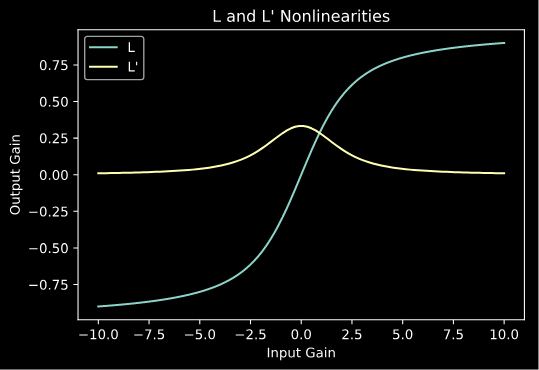
\includegraphics[height=2.5in]{../Hysteresis/Pics/LangevinPlot}
    \end{figure}
\end{frame}

\begin{frame}{Hysteresis}
    Digitize hysteresis model\footcite{Transformers_JA,DAFX-tape}
    \newline\newline
    Use $S, a, c$ as parameters
    \vspace{2ex}
    \begin{equation}
        \dot{y} = \frac{\frac{(1-c)\delta_y(SL(Q) - y)}{(1-c)\delta_xk - \alpha(SL(Q) - y)}\dot{x} + c \frac{S}{a} \dot{x} L'(Q)}{1 - c\alpha \frac{S}{a} L'(Q)}
    \end{equation}
\end{frame}

\begin{frame}{Hysteresis: Parameters}
    Saturation
    \begin{figure}
        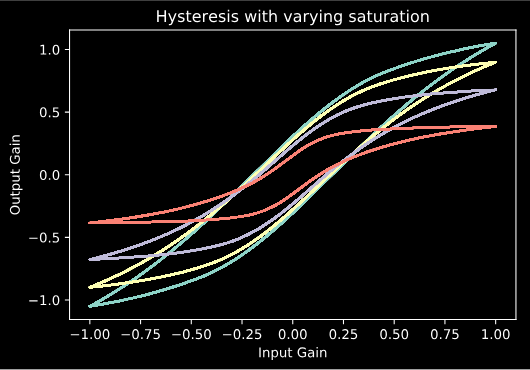
\includegraphics[height=2.5in]{../Hysteresis/Pics/Saturations}
    \end{figure}
\end{frame}

\begin{frame}{Hysteresis: Parameters}
    Drive
    \begin{figure}
        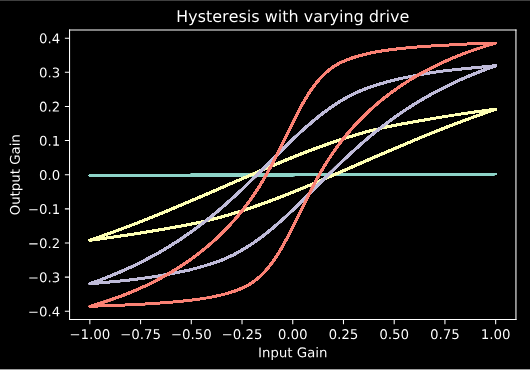
\includegraphics[height=2.5in]{../Hysteresis/Pics/Drive}
    \end{figure}
\end{frame}

\begin{frame}{Hysteresis: Parameters}
    Width
    \begin{figure}
        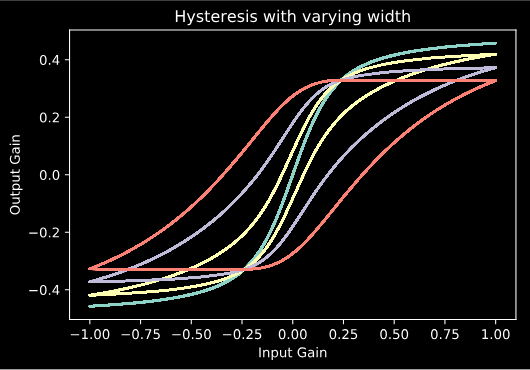
\includegraphics[height=2.5in]{../Hysteresis/Pics/Width}
    \end{figure}
\end{frame}

\begin{frame}{Hysteresis: Parameters}
    Width (with makeup gain)
    \begin{figure}
        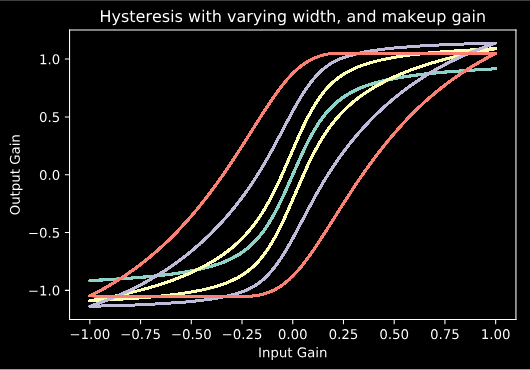
\includegraphics[height=2.5in]{../Hysteresis/Pics/Width_makeup}
    \end{figure}
\end{frame}

\begin{frame}{Hysteresis}
    \begin{columns}
        \begin{column}{0.5\linewidth}
            \begin{figure}
                \centering
                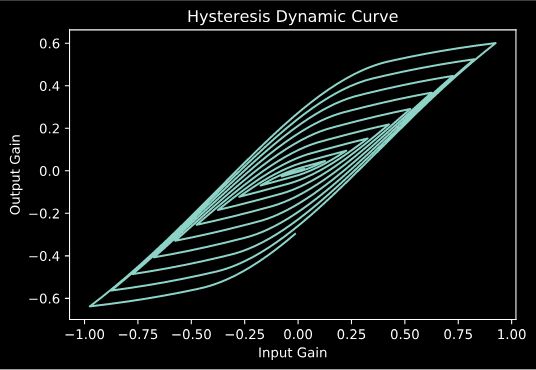
\includegraphics[width=2.75in]{../Hysteresis/Pics/Hysteresis_Dynamic}
            \end{figure}
        \end{column}
        \begin{column}{0.5\linewidth}
            \begin{figure}
                \centering
                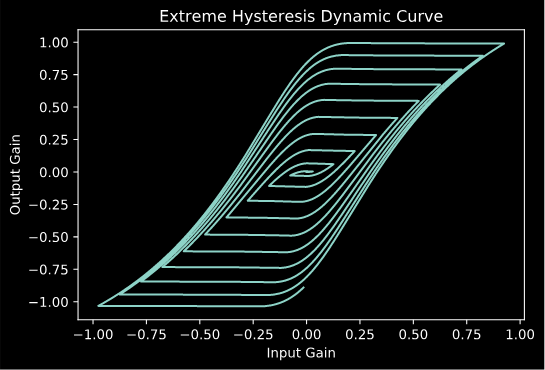
\includegraphics[width=2.75in]{../Hysteresis/Pics/Extreme_Hysteresis}
            \end{figure}
        \end{column}
    \end{columns}
\end{frame}
